% !TEX encoding = UTF-8
% !TEX TS-program = pdflatex
% !TEX root = ../tesi.tex

%**************************************************************
\chapter{Performance}
\label{cap:performance}
%**************************************************************
\section{Confronto dei vari metodi}
In questa sezione confronteremo il tempo di esecuzione dei vari metodi risolutivi per 5 configurazioni iniziali del problema, di difficoltà crescente dal livello 0 al livello 4.\\
Per i primi 4 problemi abbiamo anche un dato del tempo impiegato da una persona nel risolvere il problema. Abbiamo infatti sottoposto i vari livelli a 8 persone diverse, di età compresa tra 16 e 55 anni, cronometrandoli durante lo svolgimento del gioco.\\
Per ogni livello è presente una tabella che contiene le misure di performance, in termini di tempo medio di esecuzione, rilevate per ogni tipo di solver; inoltre tra parentesi è presente il numero medio di stati attraversati da ogni solver per arrivare allo stato obiettivo. \\
Per ogni tabella, si paragonano tra loro i risultati ottenuti da ogni solver con o senza le migliorie specificate in \ref{migliorie}

\subsection{Livello 0}
La configurazione iniziale del livello 0 è mostrata in figura \ref{lev0}. Le forme mancanti da inserire sono mostrate nelle figure \ref{z}, \ref{c}, \ref{y}.
\begin{figure}[h]
	\centering
	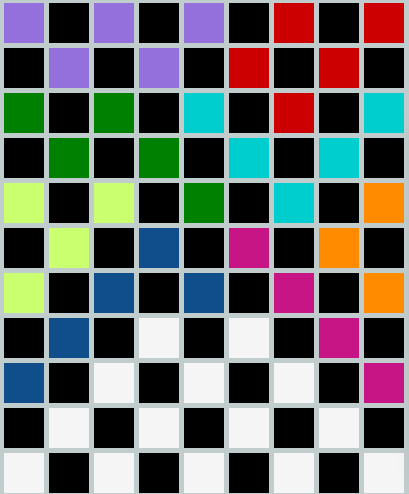
\includegraphics[scale=0.3]{immagini/lv0}
	\caption{Livello 0}
	\label{lev0}
\end{figure}
\\
\noindent

\begin{table} 
	\begin{tabular}{|l||*{4}{c|}}\hline 
		\backslashbox{Miglioria}{Solver} 
		&\makebox{DFS}&\makebox{Backtracking}&\makebox{Recursive Backtracking}	&\makebox{MinConflicts}\\ \hline 
		Sì&\textcolor{ForestGreen}{0.0107 (4.175)}&\textcolor{red}{0.0519 (11.0)}&0.0495 (11.0)&0.0129 (3.4) \\ \hline 
		No&0.0319 (24.825)&0.0178 (11.0)&0.0175 (11.0)&0.0142 (4.325)  \\ \hline 
	\end{tabular} 
\end{table}

\subsubsection{Osservazioni}
In questo livello, le forme mancanti sono solamente tre, producendo così uno spazio di ricerca molto limitato. Secondo i test effettutati e sulla base delle misure di perfomance adottate e esposte in \ref{performance}, l'algoritmo migliore risulta essere $DFS$ con la miglioria \textit{Connected Component Check} (d'ora in avanti $CCC$), mentre il peggiore risulta essere quello di $Backtracking$ con la stessa miglioria.\\

La miglioria $CCC$ permette a $DFS$ di ignorare una considerevole porzione dello spazio di ricerca. Ipotizziamo di volere inserire la prima delle tre forme mancanti, creando una componente connessa di grandezza minore della più piccola forma ancora da inserire. Senza la miglioria, l'inserimento di tale forma produrrà un assegnamento parziale dal quale non è possibile raggiungere una configurazione finale che corrisponda ad un assegnamento totale e consistente, portando quindi $DFS$ ad esplorare totalmente un cammino che è destinato a non portare ad uno stato obiettivo.\\
La miglioria, invece, si accorgerebbe subito di questo problema, potando il conseguente sottoalbero degli stati; infatti $DFS$ con miglioria attraversa in media 4,175 stati, mentre senza di essa ne attraversa in media 24,825, oscillando tra un minimo di 10 e un massimo di 30 stati.\\
Notiamo tuttavia che il tempo per arrivare alla soluzione da parte dei due tipi di $DFS$ non è proporzionale rispetto al numero degli stati attraversati (il primo numero di stati è $1/6$ dell'altro, mentre il primo tempo d'esecuzione è $1/3$ dell'altro). Questo è dovuto al fatto che il $CCC$ richiede ovviamente anch'esso un certo tempo di esecuzione, che però risulta vantaggioso ai fini dell'esplorazione dello spazio degli stati e della soluzione.\\

Per quanto riguarda il $Backtracking$ con la stessa miglioria, esso risulta essere il peggiore per il seguente motivo: notiamo come il $Backtracking$ semplice impieghi poco più del $DFS$ con miglioria, facendo quindi pensare che anch'esso sia un buon solver per questo livello di difficoltà. Tuttavia, dalla tabella si vede come il solver $Backtracking$ semplice e quello con miglioria attraversino lo stesso numero di stati, con la differenza che nel secondo viene eseguito il $CCC$, aumentandone quindi il tempo d'esecuzione.\\
Possiamo quindi affermare che a parità di stati, o se la loro differenza è poco rilevante, il solver che utilizza il $CCC$ impiegherà più tempo rispetto al suo corrispondente solver senza il $CCC$.\\

Infine, osserviamo che la miglioria \textit{Random Restart} per il solver $MinConflicts$ risulta poco utile, in quanto per la semplicità di questo livello è molto difficile che il solver si "incastri" in qualche minimo locale: nessuno dei test eseguiti per questo solver, con e senza miglioria, ha mai portato ad uno stallo in un minimo locale.
\subsection{Livello 1}
La configurazione iniziale del livello 1 è mostrata in figura \ref{lev1}. Le forme mancanti da inserire sono mostrate nelle figure \ref{z}, \ref{c}, \ref{y}, \ref{w}.
\begin{figure}[h]
	\centering
	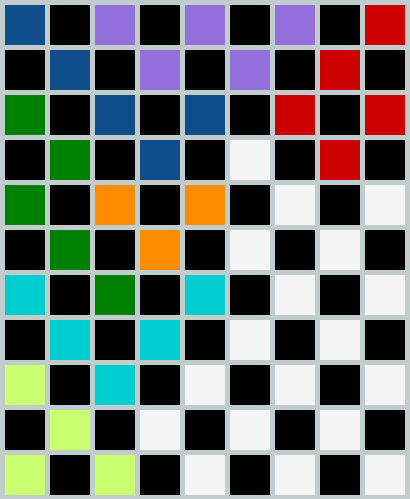
\includegraphics[scale=0.3]{immagini/lv1}
	\caption{Livello 1}
	\label{lev1}
\end{figure}
\\
\noindent
\begin{table} 
	\begin{tabular}{|l||*{4}{c|}}\hline 
		\backslashbox{Miglioria}{Solver} 
		&\makebox{DFS}&\makebox{Backtracking}&\makebox{Recursive Backtracking}	&\makebox{MinConflicts}\\ \hline 
		Sì&\textcolor{ForestGreen}{0.0271 (9.75)}&0.0666 (12.0)&0.0704 (12.0)&\textcolor{red}{0.5013 (1975.264)} \\ \hline 
		No&0.1081 (94.675)&0.0257 (12.0)&0.0270 (13.0)&0.0377 (20.82142)  \\ \hline 
	\end{tabular} 
\end{table}

\subsubsection{Osservazioni}

Per questo livello di difficoltà, i risultati ottenuti con i solver $DFS$, $Backtracking$ e \textit{Recursive Backtracking} rispecchiano quelli ottenuti nel livello 0. Non verrano quindi esposte altre osservazioni su questi solver, in quanto identiche a quelle del livello in oggetto.\\


Risulta invece necessario approfondire il significato dei valori riguardanti il solver $MinConflicts$ (rimandiamo a \ref{RR} per il significato di miglioria in questo contesto).\\
Nonostante questo livello di difficoltà possa sembrare ancora semplice, il solver \textit{MinConflicts} senza la miglioria \textit{Random Restart} (d'ora in avanti $RR$) non ha portato ad una soluzione nel $30\%$ dei test, risultando quindi di utilizzo scarsamente conveniente. \\
Con la miglioria $RR$, invece, vediamo come il tempo di esecuzione (e il numero di stati attraversati) sia nettamente più alto rispetto a qualsiasi altro solver, in quanto l'alto tasso di fallimento comporta spesso un numero elevato di riavvii dell'algoritmo, ma questo è un valore medio con una varianza troppo elevata per essere interpretato singolarmente. Risulta infatti che il numero di stati attraversati oscilli tra un minimo di 3 e un massimo di 40.376 (che corrispondono a 40 riavvii), con una maggior concentrazione intorno ai 50 stati. Quest'ultimo dato ci porta quindi a dedurre che è più probabile che il numero di stati attraversati sia qualche decina, e non diverse (decine di) migliaia.\\
Comunque sia, il solver $MinConflicts$ non è il migliore tra essi.


\subsection{Livello 2}
La configurazione iniziale del livello 2 è mostrata in figura \ref{lev2}. Le forme mancanti da inserire sono mostrate nelle figure \ref{p}, \ref{smallv}, \ref{bigz}, \ref{i}, \ref{w}, \ref{v}.
\begin{figure}[h]
	\centering
	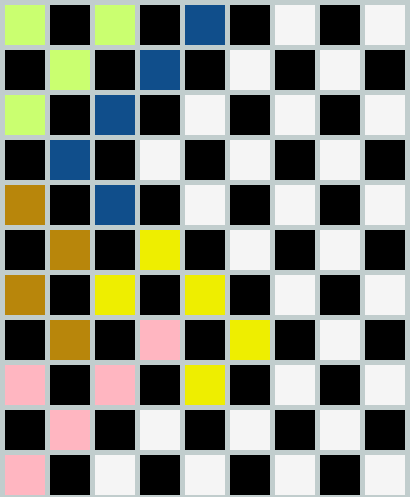
\includegraphics[scale=0.3]{immagini/lv2}
	\caption{Livello 2}
	\label{lev2}
\end{figure}
\\
\noindent
\begin{table} 
	\begin{tabular}{|l||*{4}{c|}}\hline 
		\backslashbox{Miglioria}{Solver} 
		&\makebox{DFS}&\makebox{Backtracking}&\makebox{Recursive Backtracking}	&\makebox{MinConflicts}\\ \hline 
		Sì&0.1429 (57.75)&0.1405 (22.0)&0.1227 (17.0)&\textcolor{red}{0.6263 (1414.7)} \\ \hline 
		No&1.9350 (1901.25)&0.0695 (32.0)&\textcolor{ForestGreen}{0.0579 (19.0)}&0.2054 (145.9444)  \\ \hline 
	\end{tabular} 
\end{table}

\subsubsection{Osservazioni}
In questo livello di difficoltà, il numero di forme da inserire è 6, generando così uno spazio degli stati notevolmente maggiore dei livelli precedentemente affrontati, con conseguenti osservazioni differenti.
Il solver migliore risulta infatti essere il \textit{Recursive Backtracking} senza il $CCC$, mentre il peggiore è (di nuovo) il $MinConflicts$ con il $RR$.\\

Osserviamo che $DFS$ senza $CCC$ risulta essere nettamente peggiore del suo corrispettivo con $CCC$: il tempo di esecuzione è infatti quasi 14 volte maggiore, mentre il numero di stati attraversati è circa 33 volte maggiore.\\

Per quanto riguarda il solver \textit{Recursive Backtracking} senza il $CCC$, osserviamo che non differisce di molto dal $Backtracking$ senza la stessa miglioria (infatti i tempi sono simili). Mentre, invece, essi necessitano molto più tempo per arrivare alla soluzione, se utilizzati con il $CCC$, per il motivo già spiegato nel Livello 0.\\

Le osservazioni per $MinConflicts$ risultano essere le stesse per il Livello 1, ma con parametri differenti: il solver senza il $RR$ è sorprendentemente fallito solo nel $10\%$ dei test, mentre il solver con il $RR$ attraversa un numero di stati che oscilla da un minimo di 8 ad un massimo di 16.268, con una maggior concentrazione intorno ai 150 stati attraversati.

\subsection{Livello 3}
La configurazione iniziale del livello 3 è mostrata in figura \ref{lev3}. Le forme mancanti da inserire sono mostrate nelle figure \ref{z}, \ref{smallv}, \ref{bigz}, \ref{c}, \ref{y}, \ref{t}, \ref{w}, \ref{v}.
\begin{figure}[h]
	\centering
	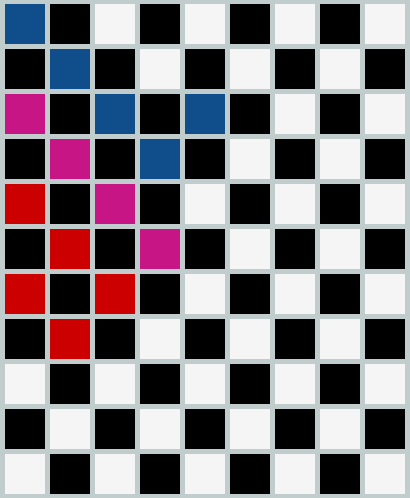
\includegraphics[scale=0.3]{immagini/lv3}
	\caption{Livello 3}
	\label{lev3}
\end{figure}
\\
\noindent

\begin{table} 
	\begin{tabular}{|l||*{4}{c|}}\hline 
		\backslashbox{Miglioria}{Solver} 
		&\makebox{DFS}&\makebox{Backtracking}&\makebox{Recursive Backtracking}	&\makebox{MinConflicts}\\ \hline 
		Sì&27.913 (8750.4)&1.0607 (198.0)&\textcolor{ForestGreen}{0.3522 (55.0)}&30.473 (65528503) \\ \hline 
		No& \textcolor{red}{30 minuti}&1.0379 (1179.0)&0.5709 (572.0)&0.1359 (36.0)  \\ \hline 
	\end{tabular} 
\end{table}

\subsubsection{Osservazioni}
Il livello 3 è il primo che presenta un grado di difficoltà elevato. Infatti il solver $DFS$ senza il $CCC$ impiega in media circa 30 minuti per arrivare ad una soluzione, ed è proprio in questo livello che si può meglio apprezzare l'utilità del $CCC$: il $DFS$ che fa utilizzo di tale miglioria impiega infatti solo 27 secondi in media per ottenere una soluzione.\\
Il solver dalle migliori prestazioni per questo problema è il \textit{Recursive Backtracking} con il $CCC$.\\

Nel solver $MinConflicts$ i dati evidenziano invece che il solver senza $RR$ è parecchio veloce, ma porta ad una soluzione solo nel $2,5\%$ dei casi.
Con il $RR$, osserviamo sono attraversati in media 65.528.503 stati (che corrispondono a 655285 riavii). Tuttavia questo numero oscilla da un minimo di 170 ad un massimo di $5,337913878*10^{16}$.
Quest'ultimo dato ci fa capire che, per questo livello, affidarsi a questo solver è un azzardo spesso fallimentare: è molto difficile che porti ad una soluzione, oppure potrebbe metterci un tempo troppo elevato. 
\subsection{Livello 4}
La configurazione iniziale del livello 4 è mostrata in figura \ref{lev4}. Tutte le forme devono essere inserite nella griglia.
\begin{figure}[h]
	\centering
	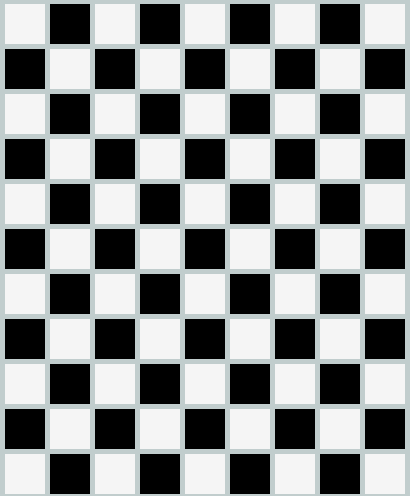
\includegraphics[scale=0.3]{immagini/lv4}
	\caption{Livello 4}
	\label{lev4}
\end{figure}
\\
\noindent

 \begin{table} 
	\begin{tabular}{|l||*{4}{c|}}\hline 
		\backslashbox{Miglioria}{Solver} 
		&\makebox{DFS}&\makebox{Backtracking}&\makebox{Recursive Backtracking}	&\makebox{MinConflicts}\\ \hline 
		Sì& ()&\textcolor{ForestGreen}{1.0781 (184.0)}&13.126 (2640.0)&17.266 (21026751) \\ \hline 
		No& ()&3.8761 (4002.0)&23.131 (23971.0)&2.0668 (796.4285)  \\ \hline 
	\end{tabular} 
\end{table}

\subsubsection{Osservazioni}
In quest'ultimo livello, il solver miglior è il $Backtracking$ con il $CCC$, mentre qualsiasi tipo di $DFS$ è ritenuto inaccettabile nel tempo di esecuzione.\\

Le osservazioni per $MinConflicts$ risultano essere le stesse per il Livello 3, ma con parametri differenti: il solver senza il $RR$ è fallito nell' $82,5\%$ dei test, mentre il solver con il $RR$ attraversa un numero di stati che oscilla da un minimo di 81581 ad un massimo di 791.975.126 .\\
Quest'ultimo dato ci fa capire che, per questo livello, affidarsi a questo solver è un azzardo spesso fallimentare: è molto difficile che porti ad una soluzione, oppure potrebbe metterci un tempo troppo elevato. 




